\chapter{System design\label{sec:tech77}}

\section{System overview}
Power Processing Unit is vital and extremely important part of the satellite.  

 According to the chapter \ref*{cha:chapter3} main requirement of the PDU is  be able to distribute a power into subsystems and payloads, which is accomplish by having a 23 power lines. Each power line controlled by a load switches which enabled by the signals from the microcontroller. Every power line measured by analog current sensors that amplify signal to the ADC that convert analog input into a digital output and communicate to the microcontroller via SPI protocol. Due to GPIO pins limitation of the microcontroller, was made a disicion to use a shift register to control additional load switches by using an I$^2$C protocol. 
 
 
  Figure \ref{fig: PDU} Illustrate the simple Power Distribution Unit architecture block diagram.\\ \\


 \begin{figure}[h]
 	\centering
 	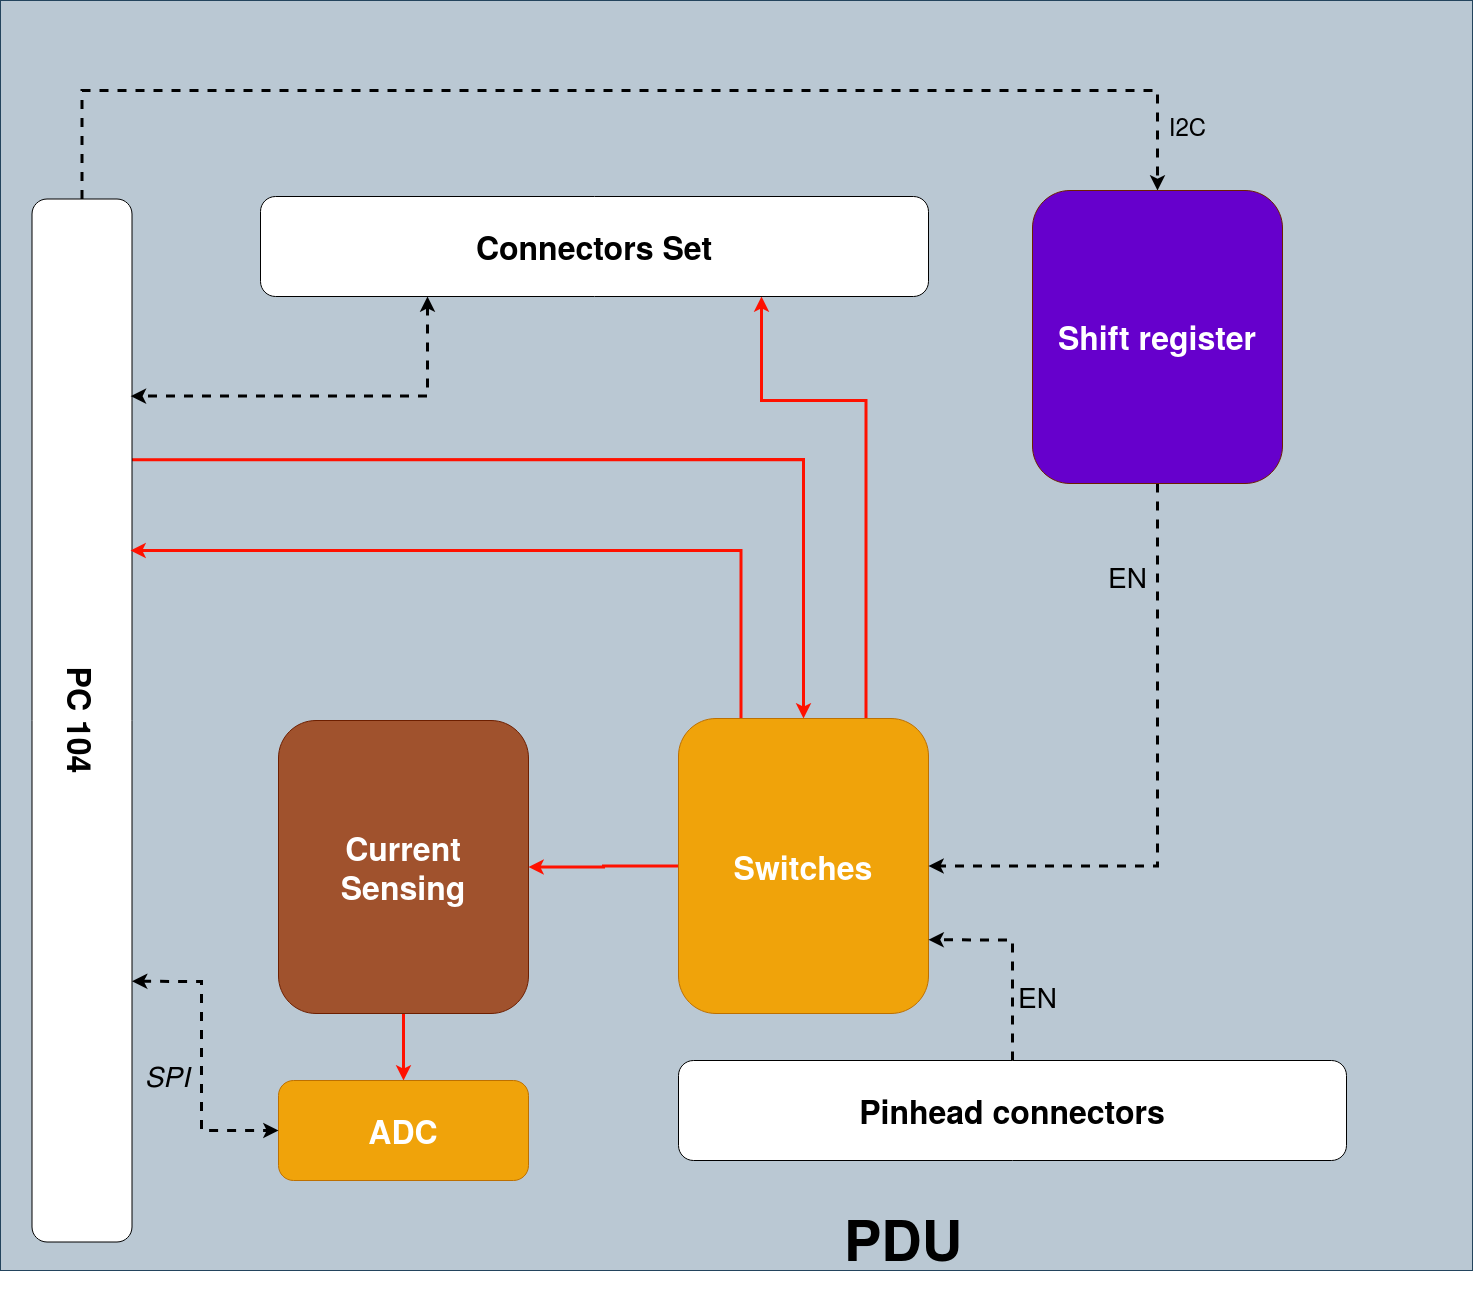
\includegraphics[scale=0.2]{PDU.png}
 	\caption{PDU board}
 	\label{fig: PDU}
 \end{figure} 

\section{Load switches}


\section{Shift register}


\section{Current sensors}

Due to the fact that PDU require to have 23 current sensors for each power line, was made a decision to use 23 analog current sensors in combination with an ADC. The main reason for that choice is to keep the flight heritage which was used for previous missions. Second reason is a relatively huge amount of sensors. Current sensors that give an output directly to I$^2$C or SPI have a limited amount of slaves which make them unsuitable to use for the current application.\\

For the Descartes mission used MAX4372T current sensor. MAX4372 is a current-sense amplifier which offer a gain of 20. MAX4372T operates on 3.3V and draws 30 µA. MAX4372 has a compact SOT23-5 package with 5 pins. Figure \ref{fig: max4372t_inside} illustrates the functionality of max4372T current sensor.

 \begin{figure}[h]
 	\centering
 	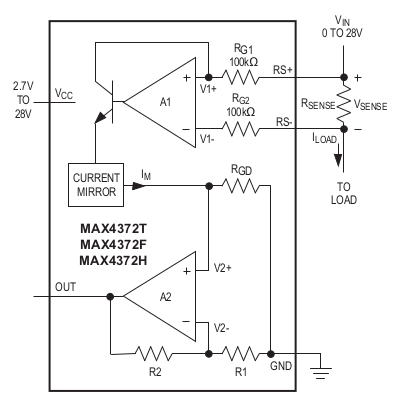
\includegraphics[scale=0.4]{max4372inside.png}
 	\caption{MAX4372T \cite{23}}
 	\label{fig: max4372t_inside}
 \end{figure} 

\cite{23}"Current flows through the sense resistor, generating a
sense voltage  Since
A1’s inverting input is high impedance, the voltage on
the negative terminal equals V IN - V SENSE . A1 forces its
positive terminal to match its negative terminal; therefore,
the voltage across $R_{G1}\times (V_{IN} - V_{1}-)$ equals $V_{SENSE}$ . This
creates a current to flow through $R_{G1}$ equal to $V_{SENSE}$ /
$R_{G1}$ . The transistor and current mirror amplify the current
by a factor of $\beta$. This makes the current flowing out of the
current mirror equal to: 

 \begin{equation}
I_{M} = \frac{\beta \times V_{sense}}{R_{G1}}
 \end{equation}
 A2’s positive terminal presents high impedance, so this
 current flows through $R_{GD}$ , with the following result:
  \begin{equation}
V_{2+} = \frac{R_{GD} \times \beta \times V_{sense}}{R_{G1}}
  \end{equation}
  R1 and R2 set the closed-loop gain for A2, which ampli-
  fies $V_{2+}$, yielding:
  \begin{equation}
  V_{out} = \frac{R_{GD} \times \beta \times V_{sense}}{R_{G1} \times (1+\frac{R2}{R1})	 }
  \end{equation}
The gain of the device equals:
  \begin{equation}
  GAIN =\frac{V_{out}}{V_{sense}} = \frac{R_{GD} \times \beta (1+\frac{R2}{R1})}{R_{G1}}
  \end{equation}
  
  MAX4372 has 3 types of current sensors, for a MAX4372T type, amplification factor equal 20.
  
  Considering different current lines and the fact that ADC has a limited tolerance of the analog input, $R_{sense}$ have to be chosen correctly according to the requirements. According to the datasheet of the ADC(MAX1231) the analog input has to be between $ -0.3V$ and $(V_{DD} + 0.3V)$ where $V_{DD}$ equals 3.3V.
  
  The value of $R_{sense}$ could be calculated with a formula:
    \begin{equation}
    R_{sense} = \frac{V_{out}}{GAIN \times I}
    \end{equation}
  
  Where:\\
  I is a current on the power line\\
  V$_{out}$ is an output voltage\\ 
 
 The table \ref{Tab:res} provide a calculated values of the shunt resistors according to the current recuirements of the power lines.
  
  
  \captionof{table}{Shunt resistor choosing}
   \begin{tabular}{p{3cm}p{3cm}p{2cm}p{2cm}p{3cm}} \toprule
   	Power channel & Load & I [mA] & $V_{out}$ [V] & $R_{sense}$ [Ohm]\\ \midrule
   VCC0 & OBC & 140 & 0.5 & 0.1\\
   VCC1 & OBC PH & 140 & 0.5 & 0.1\\
   VCC2 & ADCS & 460 & 0.5 & 0.05\\
   VCC3 & ADCS log & 0.06 & 0.6 & 0.5\\
   VCC4 & OBC 5V & 90 & 0.5 & 0.1\\
   VCC5 & OBC 5V & 90 & 0.5 & 0.1\\
   VCC6 & empty & empty & empty & empty\\
   VCC7 & empty & empty & empty & empty\\
   VCC8 & AURA & 600 & 0.5 & 0.05\\
   VCC9 & AMUR & 40 & 0.5 & 0.5\\
   VCC10 & DeCor11 & 40 & 0.5 & 0.5\\
   VCC11 & DeCor12 & 200 & 2 & 0.5\\ 
   VCC12 & DeCor21 & 40 & 0.5 & 0.5\\ 
   VCC13 & DeCor22 & 200 & 2 & 0.5\\ 
   VCC14 & DeCor31 & 40 & 0.5 & 0.5\\ 
   VCC15 & DeCor32 & 200 & 2 & 0.5\\ 
   VCC16 & ARM & 2000 & 1 & 0.02\\
   VCC17 & LORA & 200 &  0.5 & 0.1\\
   VCC18 & empty & empty & empty & empty\\
   VCC19 & Term. sens. & 10 & 0.2 & 1\\
   COM0 & UHF1 & 690 & 0.5 & 0.05\\
   COM1 & UHF2 & 690 & 0.5 & 0.05\\
   	HISP & HISPICO & 1500 & 0.5& 0.01\\ 
    \bottomrule
   	
   \end{tabular}\\ \\ \\ \\
  \label{Tab:res}
 Another important aspect to consider is the resistance of the power line. The resistance of the power line should be as low as possible to avoid voltage drop in the presence of high current. In the system design stage, voltage drop can be avoided by providing a low shunt resistor value. In accordance with current requirements, the HISP and VCC16 power channels must provide $ \ geq $ 1500mA, with a resistance of 1 Ohm the system will have a voltage drop of $ \ geq $ 1.5V, which will significantly affect the functionality of the output connected device.
 For this reason resistor values for HISPICO and ARM(antenna release mechanism) were chosen with minimal resistance.
 
  
  